Quoting @alpacaherder@ubuntu.social:
\url{https://ubuntu.social/@alpacaherder/110085255092991273} \#retoot

\begin{figure}
\centering
\pandocbounded{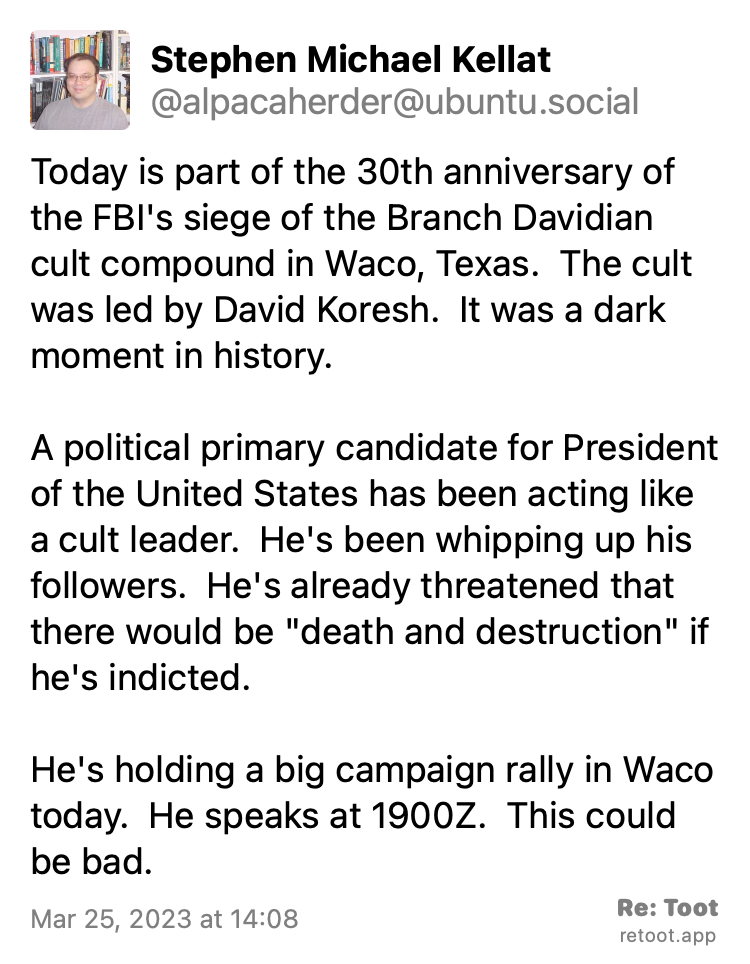
\includegraphics[keepaspectratio]{\%7B\%7Bsite.url\%7D\%7D/img/waco.jpg}}
\caption{Post by Stephen Michael Kellat. ``Today is part of the 30th
anniversary of the FBI's siege of the Branch Davidian cult compound in
Waco, Texas. The cult was led by David Koresh. It was a dark moment in
history. A political primary candidate for President of the United
States has been acting like a cult leader. He's been whipping up his
followers. He's already threatened that there would be''death and
destruction'' if he's indicted. He's holding a big campaign rally in
Waco today. He speaks at 1900Z. This could be bad.'' Posted on Mar 25,
2023 at 14:08}
\end{figure}

Well, Donald Trump had another ranting session in front of a fairly
large audience. Frankly I'm getting worried by this. His rallies are
starting to resemble Hitlerite events more and more. Increasingly
they're taking on Leni Riefenstahl sorts of production aspects.

Statements like this, as reported by
\href{https://www.theguardian.com/us-news/2023/mar/26/trump-waco-texas-2024-election-final-battle-january-6}{\emph{The
Guardian}} are not helpful:

\begin{quote}
\emph{He declared that his ``enemies are desperate to stop us'', and
``our opponents have done everything they can to crush our spirit and to
break our will. But they failed. They've only made us stronger. And 2024
is the final battle, it's going to be the big one. You put me back in
the White House, their reign will be over and America will be a free
nation once again.''}
\end{quote}

The MAGA people are being turned into an apocalyptic cult. His
campaign's kick-off rally was held in Waco, Texas. Today was the
thirtieth anniversary of the siege of the Branch Davidian compound which
was another apocalyptic cult. Anybody who lived through the 1990s here
in the United States is quite possibly still aware of that disastrous
encounter between armed law enforcement and members of a religious cult.

This passage from a
\href{https://www.newsnationnow.com/politics/trump-waco-texas-campaign-rally/}{story
by NewsNation} just bothers me:

\begin{quote}
\emph{Waco officials told NewsNation that up to 15,000 rallygoers were
expected at Waco Regional Airport for Trump's Make America Great Again
Rally.}
\end{quote}

\begin{quote}
\emph{The rally came as the U.S. nears the 30th anniversary of a deadly
siege in Waco that ended in fire and bloodshed between a cult-like group
called the Branch Davidians and U.S. and Texas law enforcement agents.}
\end{quote}

\begin{quote}
\emph{NewsNation spoke to a Republican county official who said they are
happy Trump chose Waco, though they are stumped on why he did.}
\end{quote}

\begin{quote}
\emph{The official said most politicians pick Dallas, Austin or Houston,
but said Waco is where you come to meet with the voters.}
\end{quote}

\begin{quote}
\emph{``I say to you again tonight, I am your warrior. I am your
justice,'' Trump said, echoing the message from his campaign in 2016.
``I am your retribution. We will take care of it.''}
\end{quote}

Donald John Trump holding a rally filled with apocalyptic language in
Waco on this anniversary definitely conveys a message to supporters.
Violence is the order of the day for them. This rally was a
psychological permission slip just like the one on January 6th prior to
the riot at the United States Capitol.

Reporting from
\href{https://apnews.com/article/trump-waco-rally-texas-9a5676b734bb087a977ffe0216d0a6a8}{the
Associated Press} shows in pertinent part that the Trump team may need
be occupying the same reality as the rest of us:

\begin{quote}
\emph{Trump's eyebrow-raising choice of venue in Waco for his first
rally came amid the 30th anniversary of a 51-day standoff and deadly
siege between U.S. law enforcement and the Branch Davidians that
resulted in the deaths of more than 80 members of the religious cult and
four federal agents and has become a touchstone for far-right extremists
and militia groups.}
\end{quote}

\begin{quote}
\emph{Trump's campaign insisted the location and timing of the event had
nothing to do with the Waco siege or anniversary. A spokesperson said
the site, 17 miles from the Branch Davidian compound, was chosen because
it was conveniently situated near four of the state's biggest
metropolitan areas --- Dallas/Fort Worth, Houston, Austin and San
Antonio --- and has the infrastructure to handle a sizable crowd.}
\end{quote}

That's still one heckuva coincidence to be putting forward. It is hard
to accept it is just an innocent coincidence. After all the violent
rhetoric being spewed it seems like it \emph{is not} a coincidence at
all.

That he was ranting about
\href{https://www.thedailybeast.com/trump-vows-to-defeat-demonic-forces-by-relentlessly-whining}{demonic
forces} got me very worried. He's mixing that talk about demonic forces
with
\href{https://www.cnn.com/2023/03/25/politics/trump-fact-check-waco-rally/index.html}{falsehoods
that can be debunked readily}. Is he losing his mind or is he angling to
be a martyr for a strange cult?

What Republican can knock him out in the primary? Can Biden defeat him
in the general? This is a huge mess for our country.
